


%%%%%%%%%%%%%%%%%%%%%%%%%%%
\chapter {Parallel Black Virus Decontamination in Chordal Ring}
\label{TL}
%%%%%%%%%%%%%%%%%%%%%%%%%%%
 

\section{Introduction}
In this chapter, we discuss a parallel strategy for  BVD problem in chordal rings. A chordal ring is a circulant graph with $d_1=1$, i.e., it is an augmented ring, and will be denoted by $C_n(1, d_2, ..., d_k)$. More specifically, in chordal ring each node is directly connected to the nodes at distance $d_i$ by additional links called chords. The link connecting two nodes is labeled by the distance that separates these two nodes on the ring. (see Fig.\ref{fig:chordalring})
{\bf Add a figure with an example of a chordal ring.}
\begin{figure}[H]
  \centering  
  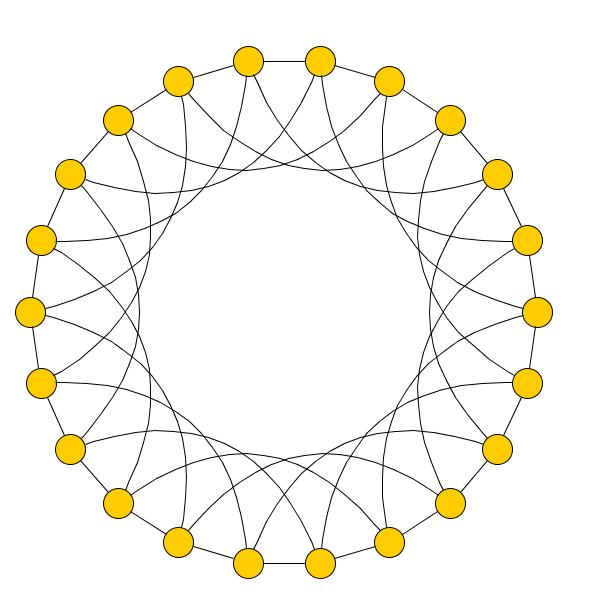
\includegraphics[width=3in]{figures/chordalring.png}
  \caption{An example of chordal ring $C_n(1,4)$}\label{fig:chordalring}
\end{figure}

%For convenience, if we say the agents or the clones move along chord $i$, then they actually move along $d_i$. If we say the agents or the clones move $i$, then they actually move along chord $d_x$ with its length equal to $i$. 
For the purpose of easier description, we assume that all the nodes in the network are marked with a number: the starting point is marked $x_0$, then the second node is marked $x_1$ \dots {\bf Do they have distinct Ids, or is this just done for the purpose of easier description ?}Agents are not allowed to communicate with each other unless they are in the same node so the protocol should enable agents in different nodes to move properly. That is, the route of every agent is different but they are served to explore the network; when a BV is triggered, other agents should bypass the new-formed BVs. We give simple but efficient solution to deal with the problem with acceptable cost. 
%Let us denote by $d$ the half degree of the chordal ring (for example, for the chordal ring structure $C_n(1,2,4,5)$, $d=4$), by $l$ the length of the longest chord of the chordal ring (for example, for the chordal ring structure $C_n(1,2,4,5)$, $l=5$). 
%{\bf d and l are already defined as $k$ and $d_k$ why change ? Use the same terminology throughout}
Our goal is to minimize the time to complete the whole decontamination process and at the same time the casualties. In order to do that, we propose a parallel strategy for decontaminating the chordal ring and this is the first attempt to deal with this issue in a parallel way. 
%
%Since time cost in the elimination phase is negligible comparing to the exploring phase if $n$ is large enough, it would be much simple to execute the elimination sequentially. That is, instead of destroy all the clones at the same time, we decontaminate them on by one. Also, in the elimination phase, in order to save the number of agents, we chase all the $Keep\,Moving$ agents (explained in section Surrounding and Elimination) back.
% It is obvious that it may cost some time for this process. If  the execution time is of great important to us and we care less the number of agents we employ, then we may carry enough agent at the beginning and start the elimination phase right after the exploring phase. 
% 

%In this Chapter we describe a single parallel strategy for the shadowed exploration phase, we then propose several different strategies for the elimination phase, each with its own advantages and disadvantages:  
%1) chasing back the $Keep\,Moving$ agents and decontaminating the BVs sequentially 
%2) chasing back the $Keep\,Moving$ agents and decontaminating the BVs parallelly 
%3) start to decontaminating the BVs right after the exploring phase and do it parallelly 
%4) start to decontaminating the BVs right after the exploring phase and do it parallelly. The cost of each strategy including time, number of agents, casualties would be analyzed in the section Analysis and Comparing.

\section{Shadowed Exploration}
\noindent{\bf Initialization }\\
The chordal ring is a complete symmetrical structure, so we can randomly choose a node $x_0$ as the start node.  The initial setup consists of deploying three groups of agents.
Initially, we place one  agent in each of the first $2d$ nodes   $x_0, x_1, \ldots , x_{2d-1}$. 
The agents residing in nodes from $x_0$ to $x_{d-1}$ form the  {\em shadowing group}, while the ones from $x_d$ to $x_{2d-1}$ form the {\em exploring group}. 
If the BV is within this window of nodes, then it is easily detected. We then assume that the  first $2d$ nodes do not contain the BV, and we place $d$ additional agents at nodes $x_ 0,x_1, \ldots, x_{d-1}$ ({\em guarding group}). 
Only the shadowing and exploring groups move to explore the graph. The ones in the guarding group remain dormant for now, guarding the nodes to guarantee monotonicity. 

\noindent{\bf Route of the agent in exploring phase}\\
The exploration proceeds in synchronized rounds composed each by  one movement step, when selected groups of agents move to proceed with the exploration, and three steps for synchronization purposes. We call these different steps    {\em move step}  and  {\em notification steps}. A round $T_i$ is composed by four time units, one for the move step, and 3 for the notification steps : 
$T_1 = T_{move\_1},T_{noti\_1},T_{noti\_1},T_{noti\_1},  
T_2 =  T_{move\_2},T_{noti\_2},T_{noti\_2},T_{noti\_2}, \ldots$.
% 
%
%$T_{move\_1}$, 
%$T_{notice\_1}$, 
%$T_{notice\_1'}$, 
%$T_{notice\_1''}$, $T_{move\_2}$, $T_{notice\_2}$, $T_{notice\_2'}$, $T_{notice\_2''}$ ...
%
%More specifically, every cycle contains one unit of time for moving and three units of time for notice. We discuss why we arrange the time as above and what exactly the agents do in the notice time later. 
The agents that move during a move step $T_{move\_i}$, always do so along their longest chord $d_k$. That is, agents move along $d_k$ in steps $T=1+4t$ $(t\in \mathbb{N})$.  
An example of how agents move in chordal ring $C_n(1, 2 , 4, 5)$ at $T_{move\_i}$ in the  exploring phase is shown in Fig.\ref{fig:subfig1}. \\

\begin{figure} [H]
  \centering 
  \subfigure[Arrangement of agents at $T_{move\_i}$]{ 
    \label{fig:subfig1:a} %% label for first subfigure 
    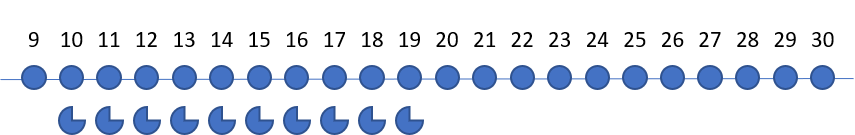
\includegraphics[width=3.0in]{figures/chordal_a_l.png}} 
  \hspace{1in} 
  \subfigure[Arrangement of agents at $T_{move\_{i+1}}$]{ 
    \label{fig:subfig1:b} %% label for second subfigure 
    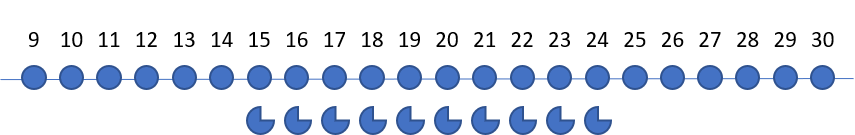
\includegraphics[width=3.0in]{figures/chordal_a1_l.png}}
  \caption{Arrangement of agents when moving} 
  \label{fig:subfig1} %% label for entire figure 
\end{figure}

\noindent{\bf Synchronization: Three\,Jump\,Notifying\,Technique}
In the sequential strategy \cite{Alotaibi}, {\bf add citation} two agents explore the graph (exploring agent and leader agent)  using  ``cautious walk". That is, the Exploring Agent moves to the next node in its route, and if the node is safe, it moves back to the Leader Explorer Agent, and then move forward to that safe node together. If instead the node contains a BV, the Leader Explorer Agent becomes aware of that because a BV arrives through that link instead of Explorer Agent. {\bf doesn't it find out by receiving the clone ?}
However, in our strategy, we employ $2d$ agents in the exploring phase but we do not use the ``casual walk". We then have to guarantee that they all find out whether or not the BV has been found in the current round. In fact, if they are not properly informed, when one agent is destroyed by the BV, in their next step some of them (the risky agents RAs) may be destroyed by the new formed BVs. In order to avoid these potential casualties, we propose the $Three\,Jump\,Notifying\,Technique$ to properly notify the agents who otherwise would move to the new formed BVs in the next round.\\

The idea is the following: when/if a node receives a clone and becomes aware of the presence of the BV,  it becomes a  $Notification\,Agent$ (NA). The NA's role is to make the risky agents aware of the presence of the BV in an efficient way. They will do so in parallel, each following  a special  route of length 3.  More precisely, let the BV be at node $x_0$ (refer to Figure \ref{fig:subfig}), the $Notification\,Agent$ located at node $x_{n-d_i}$ will follow the following route:

$x_{n-d_i}\xrightarrow [] {move\,along\,chord\,d_i}x_0\xrightarrow [] {move\,along\,chord\,d_k}x_{n-d_k}\xrightarrow []{move\,along\,chord\,d_i}x_{n-d_k+d_i}$.
 
 In this case, the notifying route of the $NA$ whose coordinate is $x_{n-d_k}$ is $x_{n-d_k}{\rightarrow}x_0{\rightarrow}x_{-d_k}{\rightarrow}x_0$.
 
 {\bf confusion between node, chord, etc. Let us always use $x_i$ for the nodes (not $i$), $d_i$ for the chords, etc..}
 
 We would make some modification of this agents route in the $Surrounding\,and\,Elimination$, but now let us assume it still follows the route above. The whole process of $Three\,Jump\,Notifying$ technique in chordal ring $C_n(1, 2, 4, 5)$ is shown in Fig.\ref{fig:subfig}. \\

%
%
%
%To explain it more clearly, let us make an example  in a chordal ring $C_n(1, d_2, \ldots,  d_k)$, assuming  for convenience that $x_0$, in this case,  corresponds to the  node containing the original BV.
%If  the   BV is triggered, its  clones  spread to nodes whose coordinates are $-d_k$, $-d_{k-1}$, \ldots, $-d_2$, $-1$, $1$, $d_2$, \ldots, $d_{k-1}$, $d_k$. 
%After a move step then, there is a risk that these nodes   are contaminated; the goal of the $Three\,Jump\,Notifying\,Technique$ 
%is to notify the agents which are supposed to move there next (the $Risky\,Agent$ ($RA$s) )   to actually stop. 
%The coordinates of the $Risky\,Agent$ ($RA$s) are $1- d_k$, $d_2-d_k$, \ldots, $d_{k-1}-d_k$, $d_k-d_k$ (which is exactly the coordinate of the original BV) respectively. It is obvious that not all of the nodes from $1$ to $d_k$ become BV nodes after the triggering because there might be some agents already there, but since notifying all the $Risky\,Agents$ does not add more cost comparing to notifying some of them, in our strategy, we notify all of the $RA$s. 

\begin{figure} [H]
  \centering 
  \subfigure[Arrangement of agents at $T_{move_i}$]{ 
    \label{fig:subfig:a} %% label for first subfigure 
    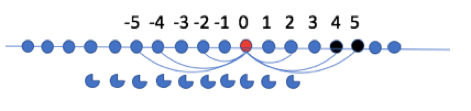
\includegraphics[width=2.5in]{figures/tjt1.png}} 
  \hspace{1in} 
  \subfigure[Arrangement of agents at $T_{notify_i}$]{ 
    \label{fig:subfig:b} %% label for second subfigure 
    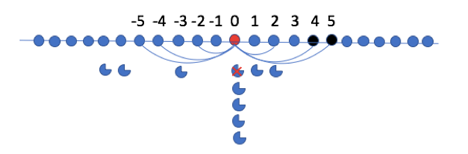
\includegraphics[width=2.5in]{figures/tjt2.png}} \
  \hspace{1in} 
  \subfigure[Arrangement of agents at $T_{notify_i'}$]{ 
    \label{fig:subfig:c} %% label for second subfigure 
    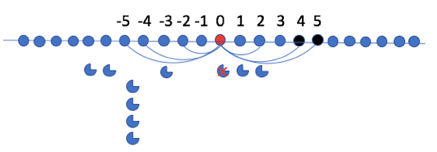
\includegraphics[width=2.5in]{figures/tjt3.png}} 
  \hspace{1in} 
  \subfigure[Arrangement of agents at $T_{notify_i''}$]{ 
    \label{fig:subfig:d} %% label for second subfigure 
    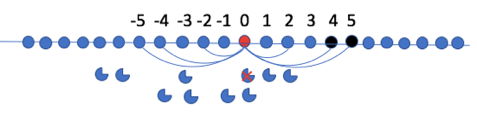
\includegraphics[width=2.5in]{figures/tjt4.png}} 
  \caption{The whole process of the $Three\,Jump\,Notifying$ technique in chordal ring $C_n(1, 2, 4, 5)$} 
  \label{fig:subfig} %% label for entire figure 
\end{figure}


If the original BV is residing in the red node, then once an agent moves to it, the agent and the BV are destroyed but the clones of the BV spread to all its neighbours. According to our technique, 
%nodes whose coordinates are $1$, $2$, $4$, $5$ become $Possible\,BV\,Nodes$; 
agents residing in nodes $-4$, $-3$, $-1$, $0$ are the  ones to be notified; 
agents residing in nodes $-5$, $-4$, $-2$, $-1$ are the $NA$s.
 The routes for agents residing in nodes $-5$, $-4$, $-2$, $-1$ are $-5{\rightarrow}0{\rightarrow}-5{\rightarrow}0$; $-4{\rightarrow}0{\rightarrow}-5{\rightarrow}-1$; $-2{\rightarrow}0{\rightarrow}-5{\rightarrow}-3$; $-1{\rightarrow}0{\rightarrow}-5{\rightarrow}-4$ respectively.\\

\noindent{\bf Safe Exploring with Three\,Jump\,Notifying technique}

After the initialization, the exploring and shadowing agents move   following the longest chord. The subsequent three time units are either used for the notification phase (if one of the agents is destroyed at  time $T_{move_i}$), or they are spent simply by waiting before the next move.
If  executing the $Three\,Jump\,Notifying$ technique,  the $NA$s move  back to where they are before the notification. For example, in the example in $Three\,Jump\,Notifying$ technique, $NA$ residing in node $-1$ moves back to node $-4$ following the reverse route in the notifying phase which is $-1{\rightarrow}-5{\rightarrow}0{\rightarrow}-4$. 

\section{Surrounding and Elimination}
 When a BV is found,  the Three\,Jump\,Notifying technique   guarantees that the risky agents are now aware of the presence of the BV. Other agents, however, might not have received the notification and might proceed to the next round without such knowledge; we call these agents $KeepMoving$ agents.   

In this section, we introduce the process of eliminating the BVs after the original BV is triggered. For the purpose of saving the number of agents, we prefer to chase the $Keep\,Moving$ agents, but it is not necessary to complete the process especially when you care most about the  execution time; In that case, we may  instead  carry enough agents  and  proceed to the $Surrounding\,and\,Elimination$ phase immediately. 
The number of agents that should be carried in order to successfully proceed the $Surrounding\,and\,Elimination$ will be discussed later.  We now describe how to chase the $KeepMoving$ agents.

\subsection{Notifying Moving Agents}

\noindent{\bf Overview of the Notifying Moving Agents}

When the $Shadowed\,Exploring$ ends, it is possible that some of the agents in the array are not informed and do not realize the existence of the BV, so they keep moving following the routes in $Shadowed\,Exploring$  phase but it is obvious that they would not encounter any BV. In order to reduce waste, we employ the agent who receives the clone from chord $d_k$ ($Coordinator\,Agent$) to notify the other $Keep\,Moving$ agents to move back to their   position  they occupied before the BV was triggered.
% Now we introduce how we choose the $Coordinate\,Agent$($CA$)and how the $CA$ notifies the other agents.\\

\noindent{\bf The Process of the Notifying Phase of the Coordination Agent}

To do that we employ one of the agents as a  $Coordinator\,Agent$($CA$). The CA follows a specific path that will guarantee to meet all the $Keep\,Moving$ within a certain amount of rounds.


The general outline of the technique is the following:
\begin{enumerate}
\item the CA is chosen to be the agent who receives a BV clone from its longest chord. %once the $Three\,Jump\,Notifying$ technique is terminated,
%\item the CA moves to occupy an arbitrary node within a special range $[y,z]$ (the rules of moving and the range computation are described later) once selected.
\item following three moving rules (the rules of moving are described later) the CA moves to occupy an node as the starting point for chasing and set a notification window $[x_y,x_z]$ (the range computation are described later) based on its own coordinate. 
\item the CA waits an appropriate amount of time to allow the agents that are still moving to reach this window of nodes
\item the CA now moves in synchronization with the movement of the agents and follows a specific paths. 
More precisely, while the moving agents proceed as usual  with one move and 3 waiting steps, the CA will take its longest chord in correspondence of an agents move and 3 consecutive nodes in correspondence of the waiting steps of the moving agents. In doing so, with $O(d_k)$ moves, the CA is guaranteed to have encountered  all of them.
\item when a moving agent encounters the CA, it stops and waits for a second agent that will arrive at the next round. When both agents are there, they go back to their original positions to start the surrounding phase.
\end{enumerate}

{\bf  ----- Now try to restructure the rest describing each of the steps in separately. }

For our convenience, in some case, we consider the chordal ring as arranged in rows of $d_k$ where the last node of a row is connected to the first node of the following row and the last node is connected to the first. Depending on the size of the chordal, the last row could be incomplete. So in this matrix, moving down a column corresponding to using the longest chord $d_k$.(see Fig.\ref{fig:matrix}). 
\begin{figure}[H]
  \centering  
  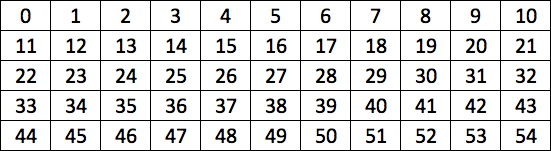
\includegraphics[width=0.6\textwidth]{figures/matrix.png}
  \caption{Viewing a chordal ring whose longest chord is 11 as a matrix}\label{fig:matrix}
\end{figure}

The selection of the $CA$ is simple: when an agent receives a BV clone from its longest chord, then it realizes that it is chosen as the $CA$. More specifically, if the coordinate of the original BV is $x_i$, then the coordinate of the CA would be $x_{i-d_k}$.
After being selected as the CA, the CA should move to an node as the starting point for chasing. 

In the following step, we would use a concept called ``notification window".  In a chord ring $C_n(1, d_2, \ldots, d_k)$, given a coordinate $x_i$, the $Notification\,Window$ $[x_y,x_z]$ based on this coordinate is set using the modular arithmetic and $x_y$ is called the $Beginning\,Flag$ while the $x_z$ is called the $End\,Flag$.
The relations between $x$, $y$, $z$ should be as follow: 
\begin{itemize}
\item $x_y$ is the biggest number which satisfies that it is smaller than or equal to $x_i$ and that $x_y$ mod $d_k$ =$0$; 
\item $x_z$ is the smallest number which satisfies that it is bigger than $x_i$ and that $x_z$ mod $d_k$ = $d_{k-1}$.
\end{itemize} 

There are three rules it should follow in correspondence to three scenarios.  

Supposing the coordinate of the original BV is $x_i$ ,the coordinates of the positions where the clones spread are: $x_{i-d_k}$ (which is the original coordinate of the $CA$), $x_{i-d_{k-1}}$, $x_{i-d_{k-2}}$, \ldots, $x_{i-1}$, $x_{i+1}$, $x_{i+d_2}$, \ldots, $x_{i+d_{k-1}}$, $x_{i+d_{k}}$.
Now we describe three scenarios:
\begin{itemize}
\item Scenario 1: The last agent of the $Exploring\,Group$ is destroyed by the BV and the positions of the clones satisfy: $x_{i-d_{k-1}+d_{k}}=x_{i+1}$, $x_{i-d_{k-2}+d_{k}}=x_{i+d_2}$, \ldots, $x_{{i-1}+d_{k}}=x_{i+d_{k-1}}$. 
\item Scenario 2: The last agent of the $Exploring\,Group$ is destroyed by the BV and the at least one pair of the positions of the clones does not satisfy: $x_{i-d_{k-1}+d_{k}}=x_{i+1}$, $x_{i-d_{k-2}+d_{k}}=x_{i+d_2}$, \ldots, $x_{{i-1}+d_{k}}=x_{i+d_{k-1}}$. 
\item Scenario 3: One of the agents in the $Exploring\,Group$ except the last agent is destroyed by the BV.
\end{itemize}

In scenario 1, the $CA$ needs to move for 5 steps to reach its destination while in the other two scenarios, it only needs to move for 4 steps to arrive the destination. Now we propose the route for each scenario.
\begin{itemize}
\item For $CA$ in scenario 1: Let us donate by $y$ the coordinate of the node in the $Notification\,Window$ set by the coordinate of the original BV which does not receive any clone and his left neighbour receives a clone (the coordinate of it is $y-1$). The $CA$ first moves to the original BV, then to node $y-1$, finally to $y$. After that it only need to move along the chord $d_k$ for twice to reach its destination.
\item For $CA$ in scenario 2: There is at least one pair of the positions of the clones does not satisfy the equations so there should be one node (assuming its coordinate is $z$) who receives a clone from the original BV but node $z+d_k$ is empty. The route now for the $CA$ is first move to the BV, then to node $z$, and then moves along the chord $d_k$ for twice to reach its destination.
\item For $CA$ in scenario 3: The $CA$ here simply need to move for one step to its right neighbour and move along the chord $d_k$ for three times to reach its destination.
\end{itemize}

In any case, the $CA$ can reach its destination within 6 unit of time which is required for the $Keep\,Moving$ agents to move to the $Initial\,Notification\,Window$, so the $CA$ start to chase the $Keep\,Moving$ agents as we introduce from $T_{notify\_{i+2}}$. 


%We know that, the notifying phase starts from $T_{move\_{i+2}}$ assuming the time when the BV is triggered is $T_{move\_i}$, which means the notifying phase begins only after all the $Keep\,Moving$ agents move twice. At $T_{move\_{i+2}}$, all the $Keep\,Moving$ agents are in a $Notification\,Window$ from nodes $d_k\times(move\_{i}+1)\,to\,d_k\times(move\_{i}+1) + d_{k}-1$, and let us donate it by $Initial\,Notification\,Window$. The $CA$ would directly move to any node in $Initial\,Notification\,Window$. Now we propose three kinds of routes for the $CA$ to move to his destination:








We can see that the relative position of agents does not change when they keep moving along the longest chord. 
For example, agents residing in nodes 1, 5, 10 (noted as $A1$, $A5$, $A10$) move along the longest chord and then $A5$ moves forward for one step. Their relative position  would be exactly the same as the situation where all of them remain dormant except $A5$ moves forward for one step. 
Now we discuss how the $CA$ notify all the $Keep\,Moving$ agents assuming they are dormant and then make some modification to fit the scenario where the $CA$ notifies the $Keep\,Moving$ agents. The problem we need to solve is that given a range within which the agents are in and a $CA$ located in this range, let the $CA$ to notify all the agents in this range. 




When the agent is chosen to be the $CA$, it computes its $Notification\,Window$. When we mention marking a flag, it does not mean that the agent has to move to the node to do that but only needs to remember the positions of the two flags in its memory. Also, after the position of the $Notification\,Window$ is set, it remains stable. More specifically, when the $CA$ moves, he does not set another $Notification\,Window$ using its new position. The $CA$ moves step by step to every possible position and notifies the agents to go back if there is one until it realizes that it just passes the $End\,Flag$. After that, he moves along the longest chord anticlockwise to the node marked a $Beginning\,Flag$ and continues moving again step by step to notify agents until it arrives its relative departing node. For example, if the $CA$ starts to notify other from node $x$, then its relative departing node is $x'=x+t\times{d_k}$ ($t\in \mathbb{N}$).

We make some modifications to let the solution fit the real scenario where the agents move along the longest chord: 
\begin{itemize}
\item The Beginning Flag and the End Flag move along the longest chord also to keep the relative position the same. 
\item  When one agent $A1$ moves to a node where there is an agent $A2$ knowing the position of the original BV, $A1$ would be informed and directly moves along the longest chord to its own position. 
\item  Let us assume that the time when the original BV is triggered is $T_{move\_i}$ ($T_{trigger}$), then the $CA$ should remember the $T_{trigger}$ and informs the agents he encounters of it. The agent $A1$ who encounters the $CA$ should remember the time when they encounter ($T_{notify\_now}$) and stop moving until next $T_{move}$ when it will meet another agent $A2$. Then $A1$ moves along $d_k$ anticlockwise for $T_{move\_now}-T_{trigger}$ times while $A2$ moves for $T_{move\_now}-T_{trigger}+1$ times. 
\item When arriving its relative departing position at $T_{move\_a}$, the $CA$ knows that it has finished the task and moves along $d_k$ for $T_{move\_a}- T_{trigger}+1$ times to its position when the original BV is triggered.
\item Let us assume that the time when the BV is triggered is $T_{move\_i}$, the $CA$ starts to move step by step to notify other agents after $T_{move\_{i+2}}$, because we want to ensure the security of the $CA$. If it starts to notify other agents at $T_{move\_{i+1}}$, it might encounter a BV. Also, it should be ensured that the $Keep\,Moving$ agents in the exploring group are in the $Notification\,Window$ of the $CA$, or the $CA$ would never encounter them. We would talk about how to ensure this in next section.
\end{itemize} 


An example of how the agents and the $CA$ move in chordal ring $C_n(1, 2, 7, 11)$is shown in \ref{fig:T29}. 
\begin{figure}[H]
  \centering  
  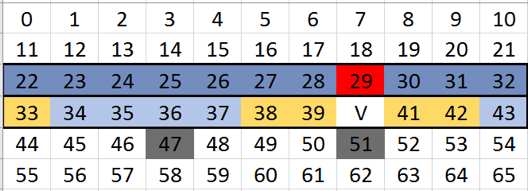
\includegraphics[width=0.6\textwidth]{figures/T29.png}
  \caption{Arrangement of agent at $T_{move\_2}$ when the BV is triggered}\label{fig:T29}
\end{figure}

Yellow nodes are connected to the original BV but guarded by agents while the grey nodes are the new formed BVs. The node marked $V$ is the original BV but now is clean. Agent residing in node 29 receives clone from chord $d_k$ so it knows it is the $CA$ During the notifying time, agents residing in nodes 33, 38, 39 notify agents residing in nodes 36, 31, 30 respectively following the $Three\,Jump\,Notifying\,Technique$ while the $CA$ moves to 28, 39, 50 and finally 61 following the route in scenario 3.

\begin{figure}[H]
  \centering  
  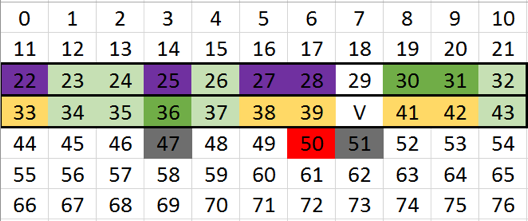
\includegraphics[width=0.6\textwidth]{figures/T50.png}
  \caption{Agents roles after $Three\,Jump\,Notifying\,Technique$ and choosing $CA$. (for convenience, we donate the $CA$ by a red spot, more specifically, node 50 is where $CA$ resides)}\label{fig:T50}
\end{figure}

Agents in purple nodes would be notified at $T_{move\_3}$ and move back. Agents in light green nodes are the $Keep\,Moving$ agents while agent in dark green nodes are informed to stop in $Three\,Jump\,Notifying\,Technique$. In the meantime, the $CA$ moves to node 28, 39, 50, and finally 61. It is obvious that the $CA$ can reach its destination before $T_{move_4}$, so it waits until $T_{notify_4}$ to start its notifying phase. 

\begin{figure}[H]
  \centering  
  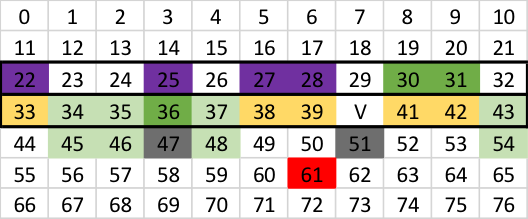
\includegraphics[width=0.6\textwidth]{figures/T611.png}
  \caption{Arrangement of agent at $T_{move\_3}$. The $CA$ has arrived its destination)}\label{fig:T611}
\end{figure}

\begin{figure}[H]
  \centering  
  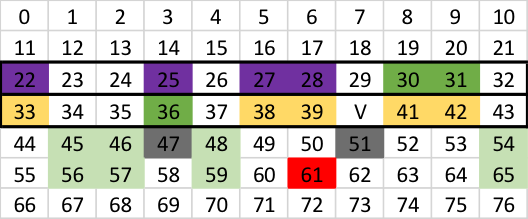
\includegraphics[width=0.6\textwidth]{figures/T612.png}
  \caption{Arrangement of agents at $T_{move_4}$. The $CA$ starts its notice phase}\label{fig:T612}
\end{figure}
In notifying phase, $CA$ starts to notify other $Keep\,Moving$ agents. First, it computes the $Notification\,Window$ which is from node 55 to node 65. Note that the $Notification\,Window$ would move along chord $d_k$ at every $T_{move}$. It moves to node 62 at $T_{notify\_4}$, node 63 at $T_{notify\_4'}$, node 64 at $T_{notify\_4''}$ and to node 75 at $T_{move\_5}$.

\begin{figure}[H]
  \centering  
  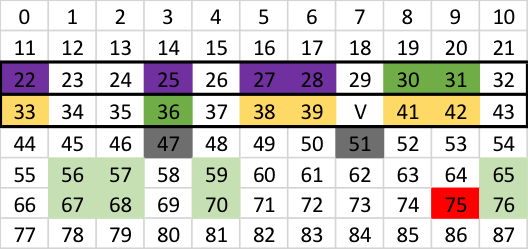
\includegraphics[width=0.6\textwidth]{figures/T75.png}
  \caption{Arrangement of agents at $T_{move_5}$. }\label{fig:T75}
\end{figure}
Again, in the notifying phase, $CA$ moves to node 76 at $T_{notify\_5}$. We can see that it encounters agent residing in node 76, so $CA$ informed it the $T_{trigger}$ which is $T_{move\_2}$. Agent residing in node 76 should remember $T_{notify\_now}$ which is $T_{notify\_5}$ and wait until next $T_{move}$ to inform agent ($Following\,Agent$) who resides in node 65 now but would move to node 76 next $T_{move}$. After encountering its $Following\,Agent$, it informs it to move back along chord $d_k$ for $T_{move\_now}-T_{trigger} +1$ times which is $T_{move\_5}- T_{move\_2}+1$ times while itself moves for $T_{move\_5}$- $T_{move\_2}$ times. 
At $T_{T_{notify\_5'}}$ when the $CA$ arrives at node 77, it knows that it just pass its $Ending\,Flag$ so it moves along the longest chord anticlockwise to its $Beginning\,Flag$ at $T_{notify\_5''}$.
\begin{figure}[H]
  \centering  
  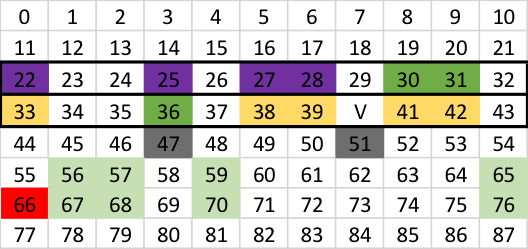
\includegraphics[width=0.6\textwidth]{figures/T66.png}
  \caption{Arrangement of agents at $T_{move_5''}$. }\label{fig:T66}
\end{figure}

\begin{figure}[H]
  \centering  
  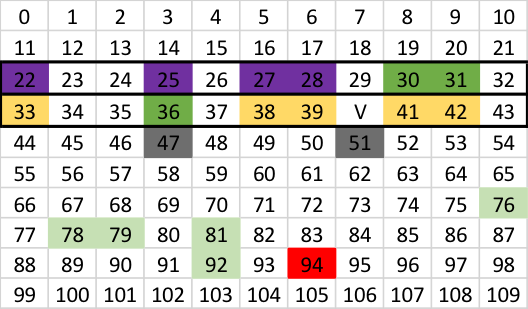
\includegraphics[width=0.6\textwidth]{figures/T94.png}
  \caption{Arrangement of agents at $T_{move_7''}$. }\label{fig:T94}
\end{figure}

We could know that the $CA$ moves back to its relative original position at $T_{notify\_7''}$. It would wait until next $T_{move}$ to inform its $Following\,Agent$ of $T_{trigger}$ and moves back with it.

\subsection{Overview of the Elimination}
After all the agents move back to where they are when the BV is triggered, we start the $Surrounding\,and\,Elimination$. We can destroy the BVs sequentially which is simple to execute but might in some case cost more time. In this way, because all the agents are aware of the positions of the new-formed BVs, so every time at most $d-1$ agents are sent to surround one of the BV and one agent is sent to destroy the BV and move on to decontaminate the second BV in a same way. Actually, this elimination strategy is the same as that in \cite{Alotaibi}. Or if we care most the execution time , we can destroy the BVs at one time. First we need to guard all the neighbouring nodes of the new formed BVs. In order to avoid collision and efficiently leverage the agents, we allocate different Destination Tables to all the agents in the array to inform them where should they should move in different situations (e.g., when the first agent in the exploring team is destroyed, then every agent except the first agent have a distinct destination, when the second agent is destroyed, then every agent except that agent destroyed have a distinct destination. More specifically, for a Chord Ring with half degree $d$, every agent in the array carries a $Destination\,Table$ with $d-1$ destinations. If we need more agents, then we will give their $Destination\,Table$ to the last agent in the shadowing group, when the elimination begins, it clones enough number of agents and give the $Destination\, Table$ to them. Before moving to its destination, the agent computes the shortest route from its own position to its destination using Dijkstra Algorithm. There are two kinds of agent in the Elimination phase: surrounding agents who are responsible for guarding the neighbouring nodes of the BVs and destroying agents who move to the BVs after all the neighbouring nodes are guarded. We want the BVs to be destroyed at one time, so it is important that the destroying agents move to the BVs at the same time and only after all the neighboring nodes are guarded by agents. In fact, if the destroying agents know the longest time $t_{longest}$ to move to the destination taken by all the agents (including the destroying agents and the surrounding agents), then they move to the last node prior to the destination and wait until $t_{longest}$ to move to the BVs together. So in the $Destination\,Tables$ for the destroying agents, we also add an item which is the $t_{longest}$. Now we introduce how to compute the shortest routes and how we design the $Destination\,Tables$. Note that we design $Destination\,Tables$ for all the agents and allocate them to the agents before the exploring phase begins.

\subsection{Destination Table and Elimination}
Supposing there are some BVs and agents in the chordal ring, it is obvious that the BV nodes are in the clockwise side of the agents. In order to use Dijkstra, first we need to map the chordal ring with BVs into a graph. We include nodes from the node containing the first agent to the node which is $d_k$ away from the last BV node, then delete the chords from the BV nodes to build the graph where we run Dijkstra Algorithm.
Here is an example how we built the graph for running Dijkstra Algorithm. Below we show the situation when the third agent in the exploring group is destroyed by the BV (see \ref{fig:D1}). Only the chords of the original BV node are shown. 
\begin{figure}[H]
  \centering  
  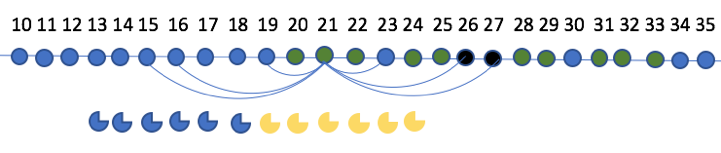
\includegraphics[width=0.6\textwidth]{figures/D1.png}
  \caption{Situation when the third agent in the exploring group is destroyed}\label{fig:D1}
\end{figure} 

The black node is the BV node while the green nodes need to be guarded. So in this case, we need 12 agents (10 surrounding agents and 2 destroying agents). 
We add nodes from 13 to 33 with their chords within this area and delete chords connected with the BV nodes to get the graph where we use Dijkstra Algorithm. Below is the graph we build. (see \ref{fig:D2}) For convenience, we show the all the nodes we included and the chords we delete.
\begin{figure}[H]
  \centering  
  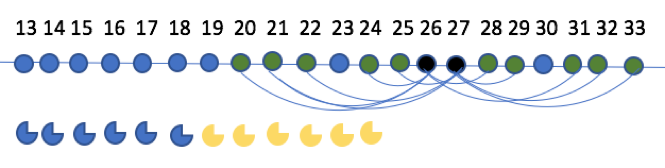
\includegraphics[width=0.6\textwidth]{figures/D2.png}
  \caption{The graph we build for Dijkstra Algorithm}\label{fig:D2}
\end{figure} 
Using the graph and Dijkstra Algorithm, we compute the routes from every agent to every node. Then we use enumeration to choose an allocation of every agents's destination satisfying: 
\begin{itemize}
\item 1) the maximum length of the route should be minimum. 
\item 2) after the allocation, in every needed position there should be exactly one agent.
\end{itemize}
After we get the optimal allocation, we record every agent?s distinct destination and the position of the third agent in the exploring group in their $Destination\,Table$. Also, we add the length of the longest chord to every destroying agent.
More specifically, here we talk about the situation when the third agent in the exploring group is destroyed. For every agent, the information we compute would be in the third part of its $Destination\,Table$ recording the position of the third exploring agent (for example, it connects this agent through chord $x$), the destination it should move if the third exploring is destroyed. For a destroying agent, there should be another item recording the length of the longest route in this part.
Above we introduce how to design one part of $Destination\,Table$ of an agent, for every agent in chordal ring, it should hold a $Destination\,Table$ of $d-1$ parts, and every part contains 2 items (for surrounding agent) or 3 items (for destroying agent).
After the one of the agent is destroyed, the agent can check their $Destination\,Table$ to get the information of their destination. Then using Dijkstra Algorithm they can compute the shortest route separately and starts to move.

\section{Analysis and Comparing}
\subsection{Theorem and Proof}
\begin{theorem}
If the structure of a chordal ring is fixed, no mater where is the BV, the number of $Keep\,Moving$ agent is a constant.
\end{theorem}
\begin{proof}


Define: Going column, the column in which the agents keep going when an explorer encounters a virus.\\
Define: Stop column, the column in which the agents stop moving when an explorer encounters a virus.
We assume that the structure of the ring is $C_n(1, d_2, d_3,\dots, d_k)$, and there are d columns in the matrix which are $M={c_0,c_1,\dots, c_{d-1}}$\\
We assume the number of node where the original BV is V($P_V$), then it should in the column $c_{v\,mod\,d}$.\\
A column  is a stop column if and only if $\exists i,j\in [1,d]$, so that $(V+r_i)\,mod\,d=S$ or $(V-r_i)\,mod\,d=S$.\\
If the explorer encounters the virus at the position $P_{V+a}$ instead of $P_V$. Since $(V+r_i+a)\,mod\,d=(S+a)\,mod\,d$ or $(V-r_i+a)\,mod\,d=(S+a)\,mod\,d$, the column $c_{(S+a)\,mod\,d}$ should be a stop column.\\
In another word, if $c_S$ is a stop column when virus position is $P_V$, then $c_{(S+a)\,mod\,d}$ is a stop column when the virus position is $P_{V+a}$.\\
We assume we have two different stop columns $c_x$ and $c_y$ , when the black virus's position is $P_V$.  So when the black virus's position is $P_{V+a}$, the columns are $c_{(x+a)\,mod\,d}$ and $c_{(y+a)\,mod\,d}$. It is obviously that $\forall a$, if $x\neq y$, then $(x+a)\,mod\,d\neq(y+a)\,mod\,d$. That means we also have two different stop columns. So that the number of stop column does not decrease, which means that given a fixed chordal ring $C$ and the number of agent keeping moving when the BV is in V (V can be any position), then the number of agent keeping moving when the BV is in other position does not decrease.\\
Let us assume that the number of agents keeping moving in different case when the longest chord remains the same is different and donates the minimum number of going columns among them by $N_{minimum}$ while the maximum number of going columns among them by $N_{maximum}$, then according to our conclusion $N_{minimum}\geq N_{maximum}$, which means that $N_{minimum}= N_{maximum}$ . In another word, the number of agents keeping moving is a constant when the structure of the chordal ring is fixed. 
\end{proof}

The second theorem is reserved for proving the number of agents needed in different strategies in elimination
 
\subsection{Analysis and Comparing}

\noindent{\bf Time cost analysis and comparing}
We only consider the situation when n (the number of nodes of the chordal ring) is much larger than $d_k$, and since the time cost in the elimination phase is $O(1)$.  Finally, we compute the TWT of both protocols to present a more fair comparison.
Let us assume that the total number of moves is $M$, then the worst case costing the most time is when the BV is located at any nodes with number from $n-d_k+1$ to $n-1$ and the first agent (anticlockwise) is in the node with the number $n-d_k$. In this case, it cost $M=\left \lfloor \frac{n}{d_k}-1\right \rfloor$ moves and 4$M$ units of time (4$M=4\times \left \lfloor \frac{n}{d_k}-1\right \rfloor$) to finish the exploring phase. 
In \cite{Alotaibi}, she give the number of move in three case.
\begin{itemize}
\item 1) In double loops the upper bound of moves is $4n-7$.
\item 2) In the triple loops, she discusses two classes of chordal ring: $C_n(1,p,k)$ and $C_n(1,d_k-1,d_k)$.In the first case, the number of moves needed is $5n-6d_k+22$ while in the second case, a maximum of $5n-7d_k+22$ moves are needed.
\item 3) In the consecutive-chordal rings, a maximum of $(d_k+2)n-2d_k-3$ moves are needed.
\end{itemize}
Since in the sequential strategy, agents do not need to wait so the time cost is equal to the number of moves. And it is obvious that our protocol is much faster than the sequential strategy. But since we use much more agents, so in order to gain a fair comparison, now we compute TWT of both protocol.
In the exploring phase, we use $2d_k$ agents, so the TWT of our protocol is $8n-8d_k$. In the exploring phase of the sequential strategy, it need at least 2 agent to explore and some other shadow agents to guard the explored nodes but the number of shadow depends on the structure of the chordal ring so now we ignore them. Now we compute TWT of the sequential strategy.
\begin{itemize}
\item 1)In double loops the upper TWT is $8n-14$
\item 2)The TWT in chordal ring $C_n(1,p,d_k)$ is $10n-6d_k+44$ and in chordal ring $C_n(1,d_k-1,d_k)$ is $10n-14d_k+44$.
\item 3)The TWT in consecutive-chordal rings is $2(d_k+2)n-4d_k-6$.
\end{itemize}
It is obvious that when $d_k\geq 2$, our protocol is faster in first case; when $d_k\leq \frac{1}{3}n+7$,our protocol is faster in the second case (both $C_n(1,p,k)$ and $C_n(1,d_k-1,d_k)$); when $d>2-\frac{1}{n+2}$, our protocol is faster in the third case.

\noindent{\bf Calamity Analysis}
Casualty is the number of agents destroyed by the BV. In chordal ring $C_n(1, d_2,\dots, d_k)$, the worst case is that the first agent in the exploring group is destroyed by a BV and the clones of it spread to all its neighbouring nodes. The casualties in this case are $d_k+1$ because another $d_k$ nodes are guarded by agents while in sequential case, the casualties are $2d_k$. So in terms of casualty, our protocol is better than the sequential strategy.

Following part are reserved for analysis for different strategy in elimination: including proposing function to calculate the exact cost of different strategies...





